\chapter{系统与外设}

\hypertarget{ux7cfbux7edfux79fbux690d}{%
\section{系统移植}\label{ux7cfbux7edfux79fbux690d}}

受限于实力及时间,目前\texttt{EasterMips}仅成功进行了\texttt{PMON\ for\ LS1B}
,\texttt{Ucore}
的正常启动。对于\texttt{Linux},只完成了内核态的初始化流程,在\texttt{ramdisk\_excute\_command}
执行 \texttt{/sbin/init}进入用户态时,会因不明原因发生\texttt{Panic}。
外设方面,我们进行了\texttt{NT35510\ LCD}屏幕的初始化加载及\texttt{linux}驱动移植,但受限于进度,我们暂时无法测试移植驱动的工作情况。
以下固件的编译均于如下环境下进行:

\begin{enumerate}
\item
  龙芯提供的gcc-4.3-ls232(mipsel)
\item
  Ubuntu 18.04 64bit
\end{enumerate}

同时,由于\texttt{EasterMips}暂未支持\texttt{MIPSr1}中的部分指令,故编译时使用\texttt{-mno-branch-likely}去除\texttt{branch-likely}指令,同时将\texttt{cache}等指令实现为空。

\hypertarget{pmon}{%
\subsection{Pmon}\label{pmon}}

在进行Pmon移植时,Github的编译指导带来了关键帮助:帮助定位目标设备为\texttt{LS\_1B},避免了因目标设备选择错误导致的诸多问题。
其次,在移植过程中存在\texttt{gzrom}反汇编内容主要为压缩数据,进而无法查看指令的困难。经过查找编译过程的中间文件,我们发现未压缩的\texttt{PMON}位于\texttt{Targets/LS1B/complie/ls1b}文件夹下,通过对该文件进行反汇编,调试得以正常进行。在调试中,\texttt{EasterMips}处理了如下两个较为典型的问题:

\hypertarget{badblocksux89e3ux51b3}{%
\paragraph{badblocks}\label{badblocksux89e3ux51b3}}

在初期移植过程中,启动扫描储存器时经常出现异常多的\texttt{badblocks}。在当时因未影响进行后续调试,故并没有研究该问题。而在后续对\texttt{icache}的重构中,该问题时隐时现。经过推断,该问题与可能与取指过程有关,但由于未能抓取明确波形,我们仅将其视为\texttt{icache}出错的警告信号。并通过该现象多次将取指出错的隐患迅速解决。

\hypertarget{ux7f51ux7edcux65e0ux6cd5ux4e0aux7ebf}{%
\paragraph{网络无连接}\label{ux7f51ux7edcux65e0ux6cd5ux4e0aux7ebf}}

\begin{figure}[ht]
	\centering
	\subfloat[截图 1]{
		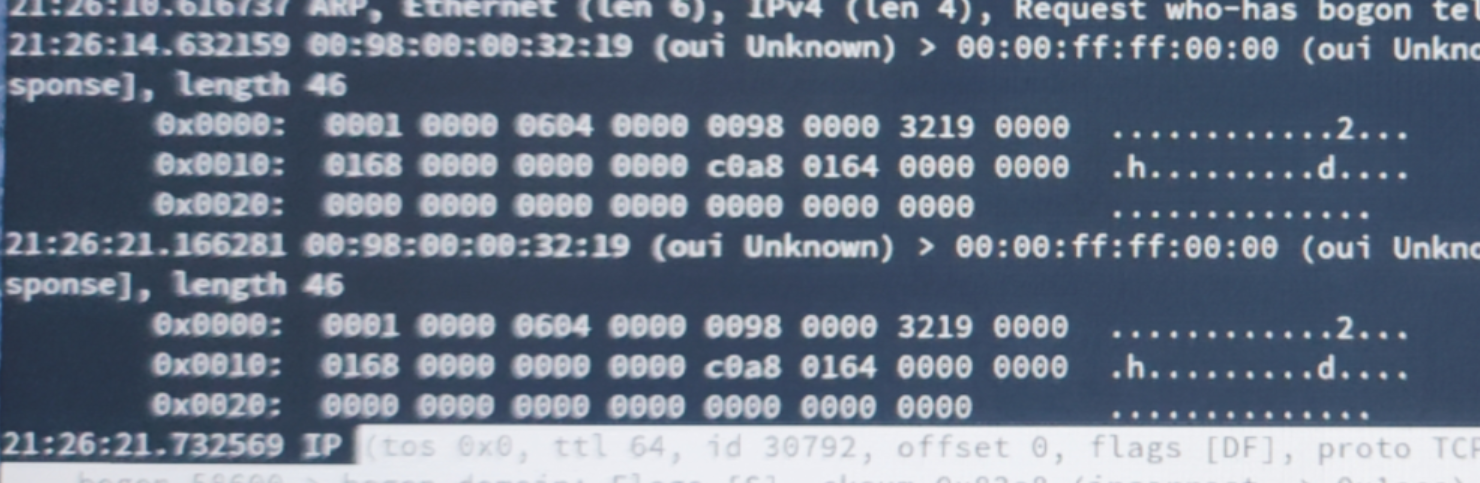
\includegraphics[width=0.4\textwidth]{network_debug_1}
		\label{fig:network-debug-1}
	}
	\quad
	\subfloat[截图 2]{
		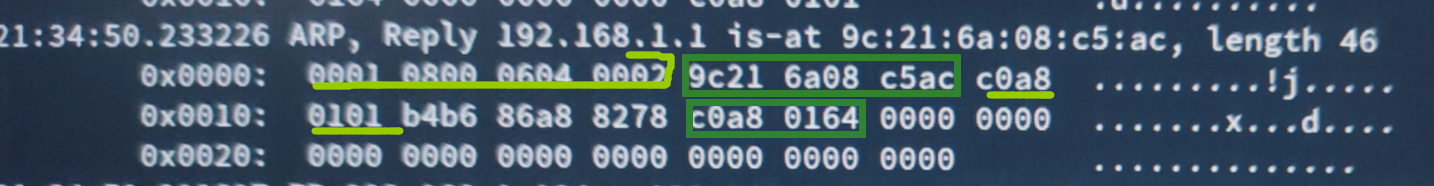
\includegraphics[width=0.4\textwidth]{network_debug_2}
		\label{fig:network-debug-2}
	}
	\caption{PMON网络调试}
	\label{fig:network-debug}
\end{figure}

在移植完成后的一次时序优化中,由于忽略了数据前递的部分条件导致\texttt{PMON}的网络无法正常加载。具体表现为\texttt{swl}与\texttt{swr}同时执行时,会丢失前者的数据。该问题的调试过程非常有趣:
在调试中首先通过\texttt{Linux}的\texttt{tcpdump}应用监听局域网可以发现,配置网络时\texttt{PMON}会发出一个无法识别的数据包,这说明写入寄存器配置的过程应当是执行无误的。其次,观察发现该数据包每32位的后16位都为全0。

考虑到其格式非常类似\texttt{ARP}数据包,我们将其与正常工作时进行了比对。如图 \ref{fig:network-debug} 中所示。有理由假定\texttt{{[}0x0,0x10{]}}是由CPU写入的,出现了异常。而\texttt{0xc0a80168}则是配置的\texttt{192.168.1.104}地址16进制数据,不经过该段程序。故我们针对性地对此类问题进行了查找,并解决了问题。

\begin{figure}[ht]
	\centering
	\subfloat[PMON运行截图]{
		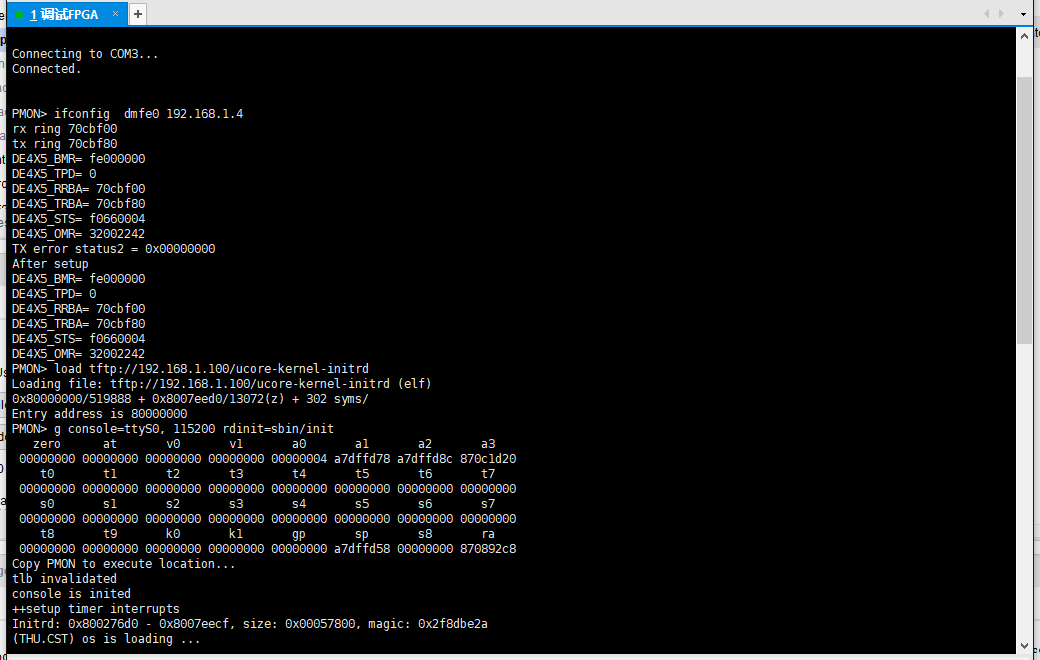
\includegraphics[width=0.4\textwidth]{PMON}
		\label{fig:pmon}
	}
	\quad
	\subfloat[Ucore运行截图]{
		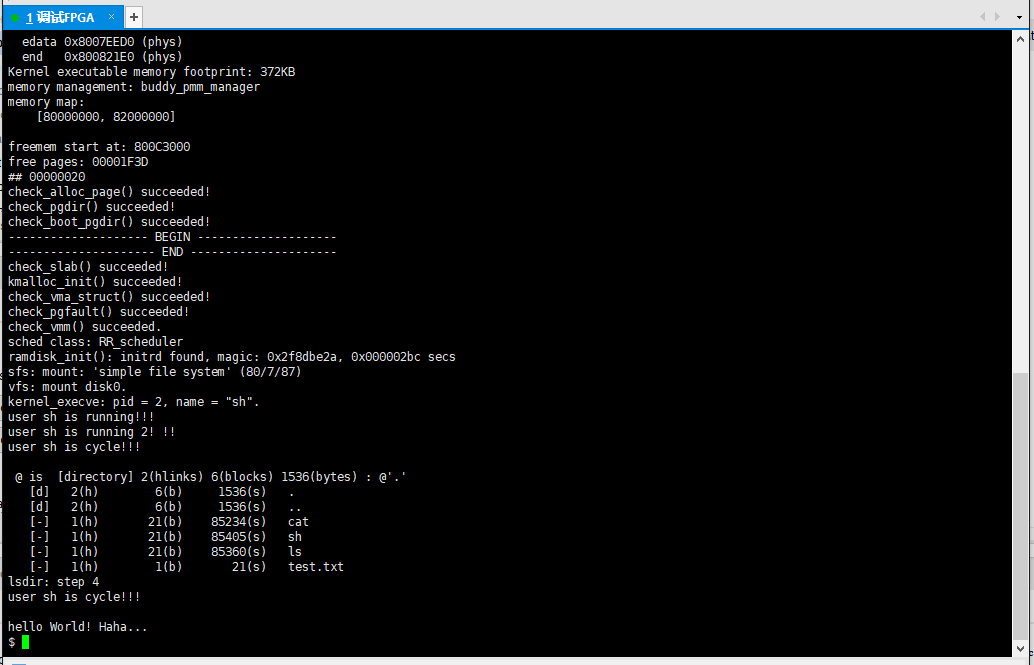
\includegraphics[width=0.4\textwidth]{Ucore}
		\label{fig:ucore}
	}
	\caption{PMON与Ucore的运行截图}
	\label{fig:pmon-and-ucore}
\end{figure}

\hypertarget{ucore}{%
\subsection{Ucore}\label{ucore}}

\texttt{EasterMips}在进行\texttt{Ucore}移植的过程中,主要帮助CPU部分进行\texttt{CP0}相关寄存器的实现及修改,并标准化诸如初始值和默认赋值、操作等实现。在进行移植的过程中,主要出现过如下问题:

\hypertarget{ux542fux52a8ux7a0bux5e8fux5f02ux5e38}{%
\paragraph{启动引导异常}\label{ux542fux52a8ux7a0bux5e8fux5f02ux5e38}}

在初次遇到问题时,我们直接使用了官方提供的 ucore
而非自己编译的内核进行引导。在执行时触发了PMON的异常,直接跳转到
\texttt{.v200\_msg}段。经过反汇编发现官方给出的ucore存在的一个直接跳转,与我们后续自行编译的跳转不符。
我们猜测这是由于面向\texttt{Rom}与面向\texttt{Ram}构建的不同,重新构建后程序正常进入启动流程。
同时在启动后续过程中,还存在系统会跳转到PMON的异常处理程序的异常行为。检查波形后我们发现这是我们没有正确实现\texttt{CP0-Ebase}寄存器导致的。

\hypertarget{ux5185ux6838ux9519ux8befux4e2dux65ad}{%
\paragraph{内核错误中断}\label{ux5185ux6838ux9519ux8befux4e2dux65ad}}

在启动初期,\texttt{++interupt\ timer}之后系统会直接陷入\texttt{trap},我们在此抓取了波形,并定位到系统在此时不应受理中断请求,但是没有被屏蔽掉。该问题耗费我们了很多时间用来debug硬件错误,直到多次检查源码后注意到
\texttt{kern\textbackslash{}trap\textbackslash{}trap.c} 文件中的
\texttt{interrupt\_handle()}在处理中断时没有考虑到\texttt{CP0-Status}寄存器,该问题导致了系统总是产生错误中断并打断启动流程。
该问题提醒我们处理故障时不能仅考虑硬件问题,也应该考虑系统驱动的问题。修改代码后系统正常运行到下一步。

\begin{figure}[ht]
	\centering
	\subfloat[截图 1]{
		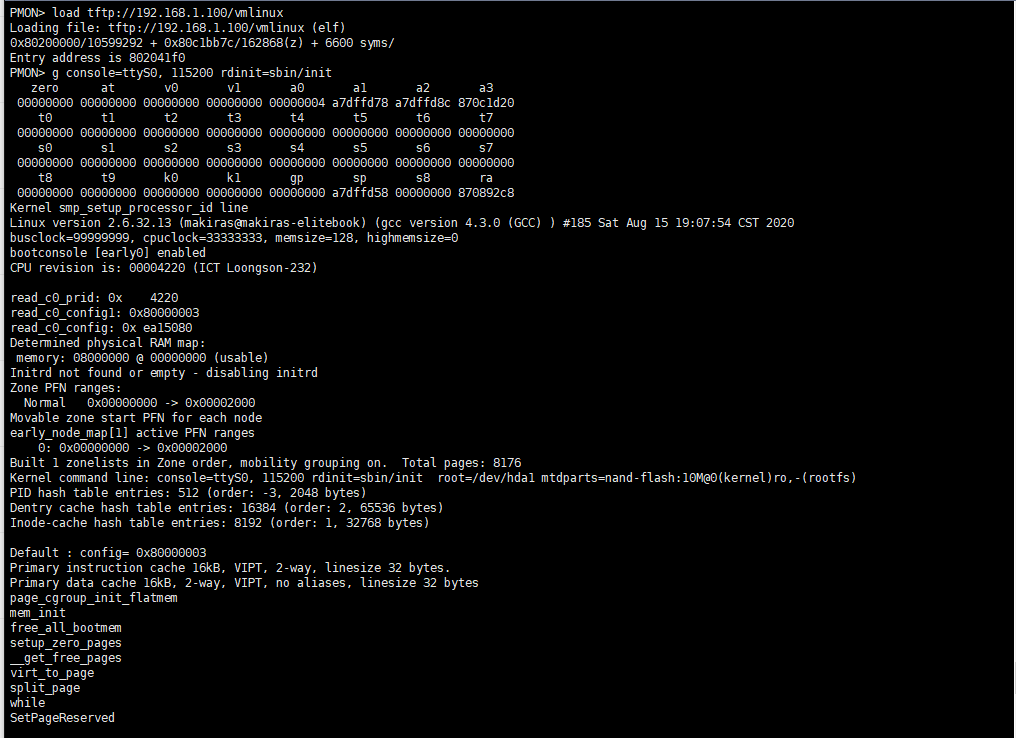
\includegraphics[width=0.4\textwidth]{Linux1}
		\label{fig:linux-1}
	}
	\quad
	\subfloat[截图 2]{
		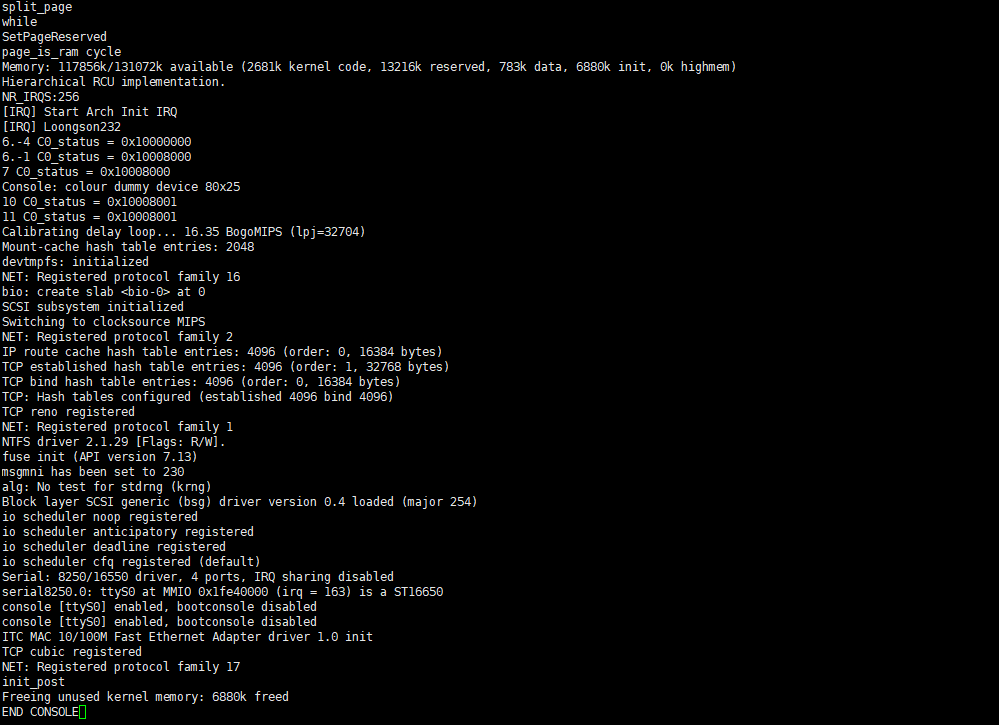
\includegraphics[width=0.4\textwidth]{Linux2}
		\label{fig:linux-2}
	}
	\caption{Linux运行截图(仅完成内核态初始化)}
	\label{fig:linux}
\end{figure}

\hypertarget{linux}{%
\subsection{Linux}\label{linux}}

在进行Linux移植的过程中,我们遇到了诸多困难。查阅参考资料后我们的移植解决了下列问题。

\hypertarget{ux6307ux4ee4ux96c6ux88c1ux526a}{%
\paragraph{指令集裁剪}\label{ux6307ux4ee4ux96c6ux88c1ux526a}}

初期调试\texttt{ucore}的过程中由于我们还未实现\texttt{tlbwr}指令,我们选择利用软件进行模拟。而在调试\texttt{Linux}时由于\texttt{build\_tlb\_refill\_handler}函数的存在,软件模拟存在不可靠和难以调试的问题,故我们补充实现了该指令。
通过在\texttt{arch/mips/include/asm/} \texttt{longson-ls1x/cpu-feature-overrides.h}中定义\texttt{cpu\_has\_llsc/ejtag/fpu}等选项,我们屏蔽了系统调用\texttt{LL/SC}指令,减少了一定的工作量。
对于自陷指令\texttt{TNE,\ BREAK}等,我们选择在\texttt{.../asm/bug.h}文件中删除相关的指令,进而绕过该问题。然而在实际操作中,该问题增加了手动Debug的难度,有许多信息需要手动设置\texttt{printk}。每次调试都需要重新加载,而PMON仅能以\texttt{260K}左右的速度加载\texttt{10M}左右的内核,这十分消耗时间。如果实现该指令,极有可能减少大量调试时间。

\hypertarget{buildrootux5236ux4f5cramdiskux6587ux4ef6}{%
\paragraph{BuildRoot制作Ramdisk文件}\label{buildrootux5236ux4f5cramdiskux6587ux4ef6}}

由于系统自带的\texttt{ramdisk.cpio}文件未提供源代码,其中含有许多我们没有实现的指令,我们需要修改\texttt{ramdisk}文件。考虑到通过反汇编修改难度过高,故最终决定利用\texttt{buildroot}工具制作我们自己的\texttt{ramdisk}文件。虽然由于时间问题在\texttt{EasterCPU}上没有成功进行初始化,但至少已在\texttt{SOC\_UP\_33M}上确认实现了正常运行,提供了简单的登录认证和性能监控。
在制作过程中,我们在最顶层\texttt{makefile}文件中始终找不到\texttt{CFLAGS}等编译参数的配置,通过全局搜索,我们才发现该参数实际处在\texttt{packages}目录下。添加编译选项后,我们确认该方法成功解决了\texttt{ramdisk}中含有不受支持指令的问题。

\hypertarget{ux5916ux90e8ux914dux7f6eux95eeux9898}{%
\paragraph{外部配置问题}\label{ux5916ux90e8ux914dux7f6eux95eeux9898}}

在进行调试时,\texttt{EasterMips}启动过程在\texttt{Calibrating\ Delay\ Loop}受阻,查阅资料我们得知这是利用定时器中断估计CPU性能的函数,进而定位问题是由于时钟中断信号所致。但由于前期在调试\texttt{soc\_up}时误将\texttt{IP7}中断有效信号误解,将除其之外的整体中断信号取反。最终导致在\texttt{ucore}在启动过程的最后无法正常输入指令,而\texttt{Linux}会卡在串口初始化。该错误操作导致的后续问题花费我们大量的时间去检查。但也因此发现了开启了内核的\texttt{no\ reconfig\ serial}默认选项后,串口波特率并不会改变,即官方提供的内核启动参数中,\texttt{115200}并不是必选项。
在调试末期,\texttt{EasterMips}还存在\texttt{Linux}初始化时的TLB异常循环问题。经过引出\texttt{k0,k1}寄存器的信号读取,我们发现在读取页表的偶数页时,访存并载入\texttt{CP0\_EntryLo0}的数据始终为0。该问题检查的检查耗时两天,直到检查\texttt{.config}文件时,我们发现系统设置的页大小为\texttt{16KB},这可能是中途编译时重新读取了\texttt{ls232\_defconfig},而未\texttt{make\ clean}所致的问题。更改为\texttt{4KB}后\texttt{EasterMips}正常进入下一步\texttt{ramdisk}初始化读取。
此类问题都是容易出问题的外部配置问题,在调试内核及CPU代码时很容易导致定位问题错误,浪费大量时间导致进度滞后。这也从侧面说明了代码习惯及行为记录的重要性。

\hypertarget{ux5916ux8bbeux6dfbux52a0}{%
\section{外设添加}\label{ux5916ux8bbeux6dfbux52a0}}

\hypertarget{lcdux5c4fux5e55}{%
\paragraph{LCD屏幕}\label{lcdux5c4fux5e55}}

我们仅在大赛官方提供的\texttt{soc\_up\_33M}上添加了\texttt{NT35510}的显示支持,通过将图片载入为\texttt{.coe}文件,我们令屏幕成功初始化。其控制接口实例位于控制寄存器模块内。
后续的\texttt{Linux}内核驱动移植因无法确认有效性,故不再进行更多描述。

\begin{figure}[htbp]
	\centering
	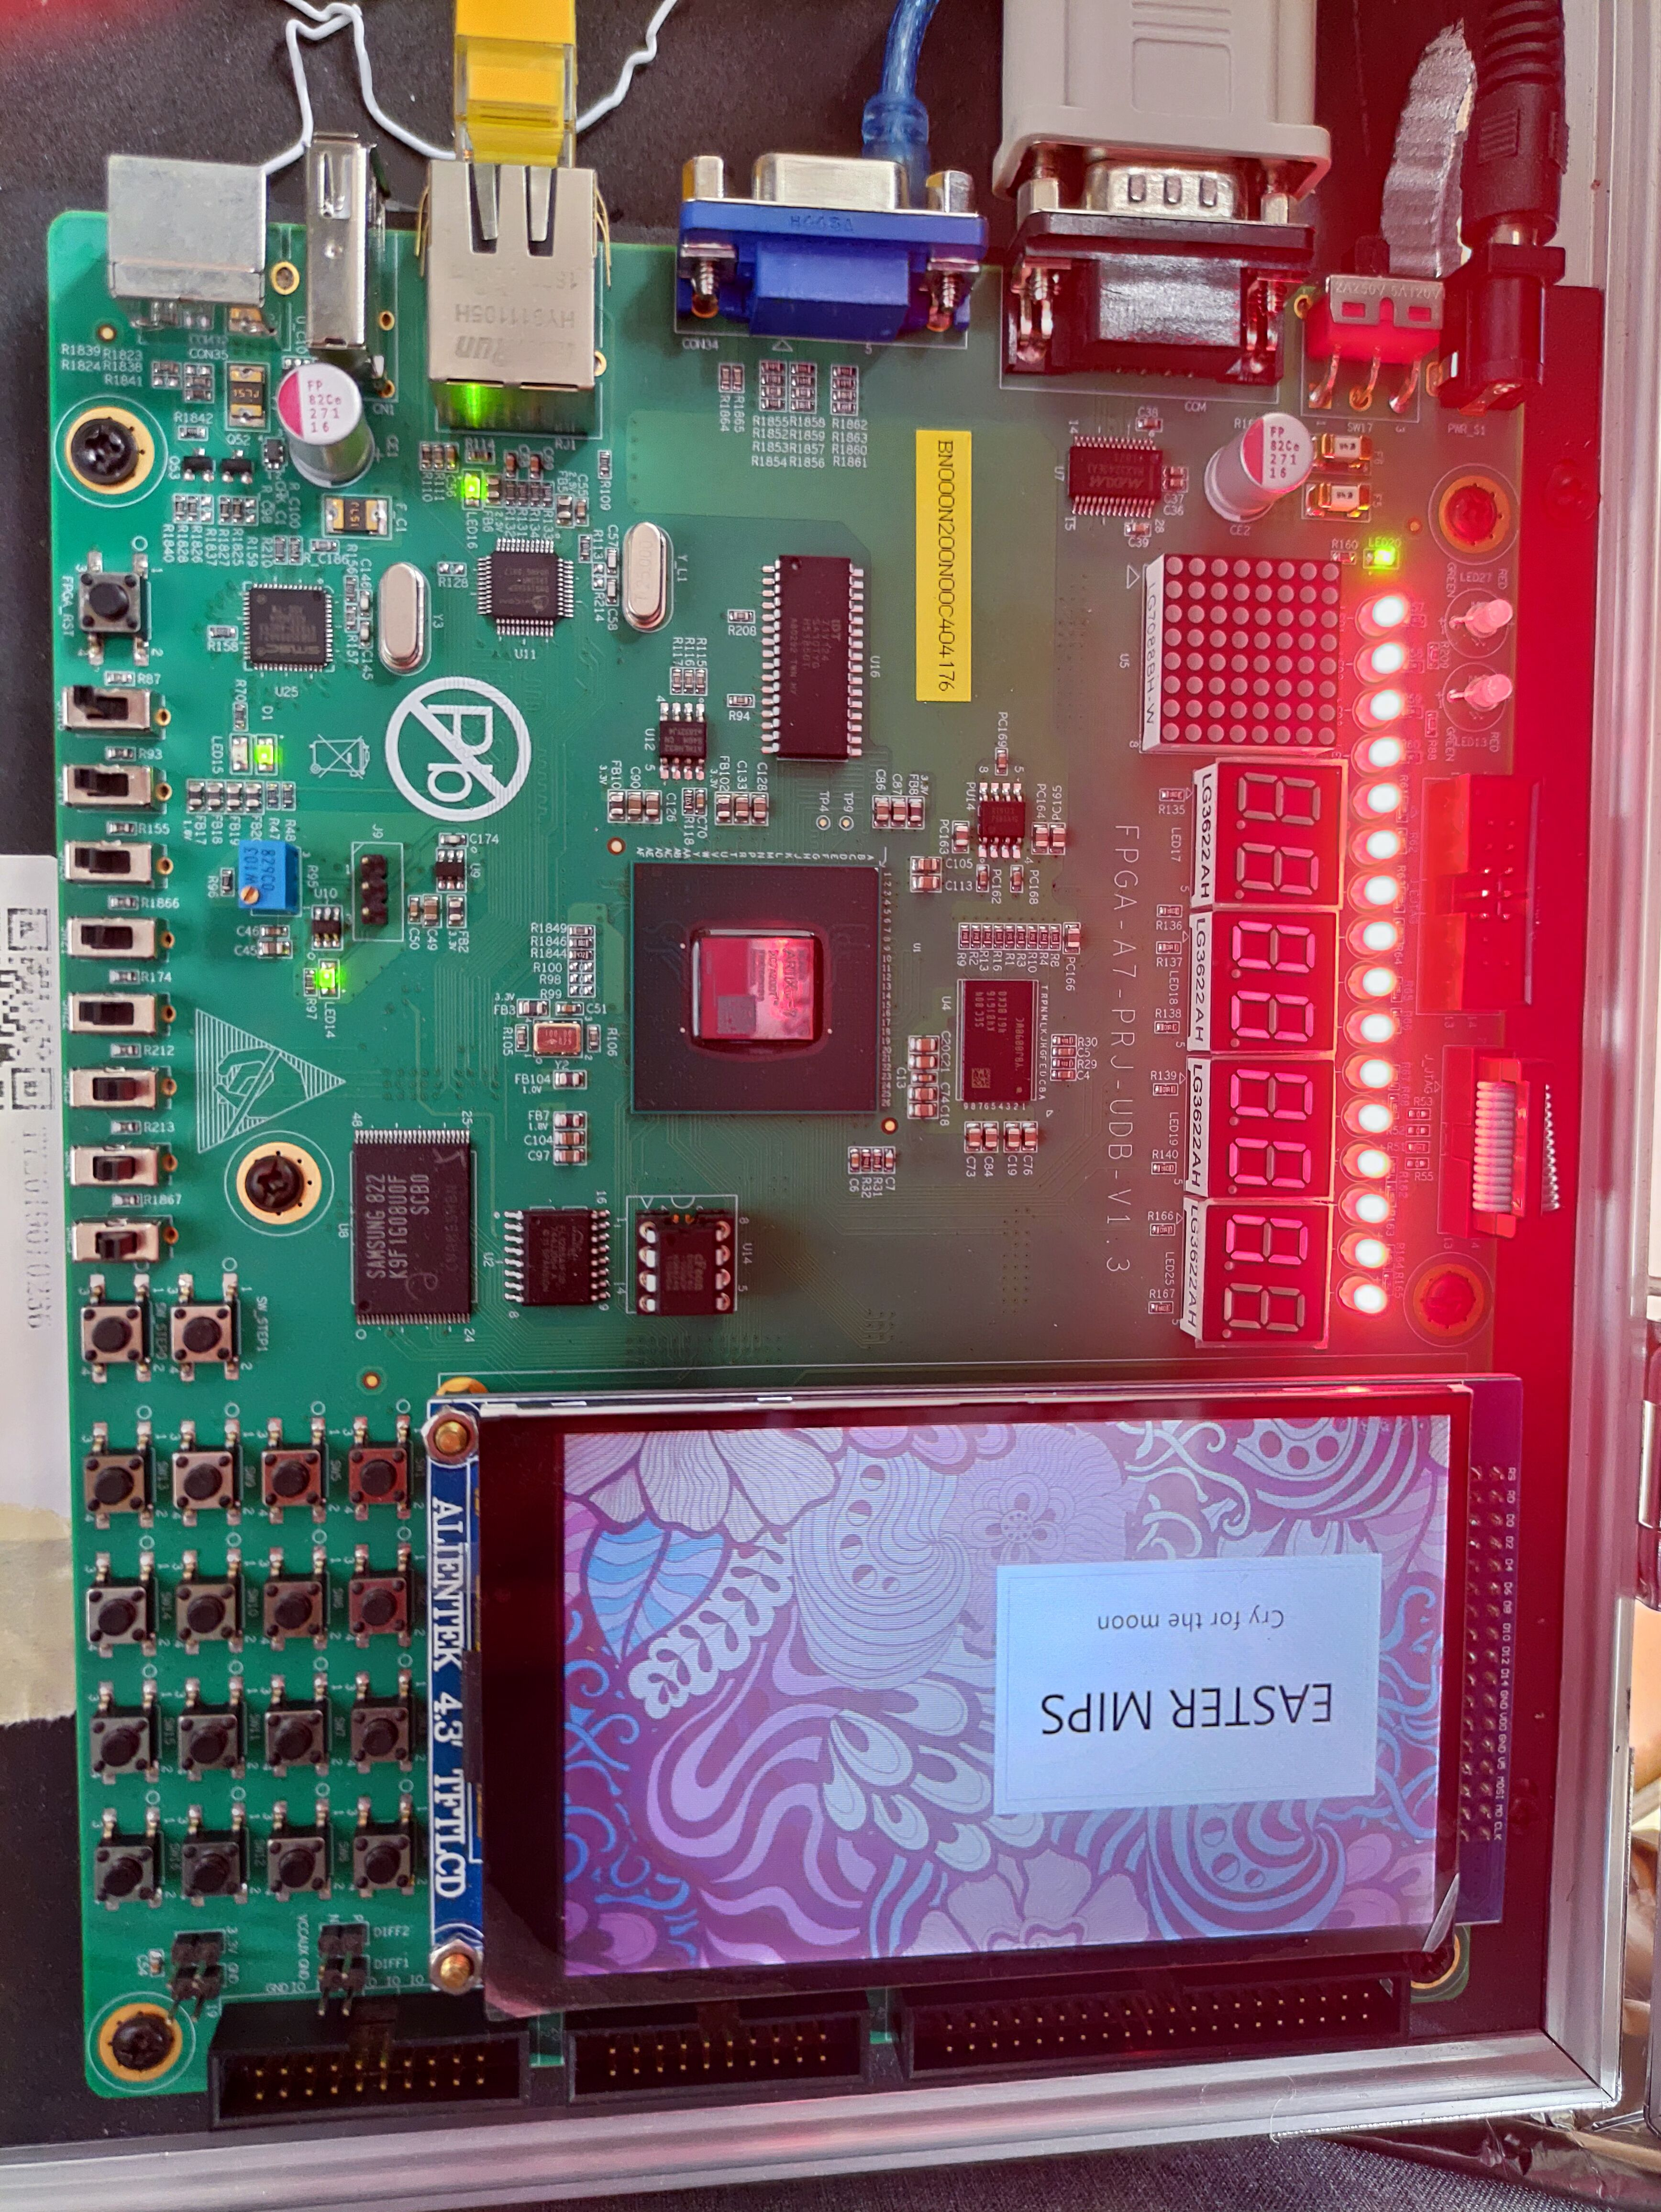
\includegraphics[angle=90,width=0.7\linewidth]{lcd}
	\caption{LCD屏幕显示}
	\label{fig:lcd}
\end{figure}

\hypertarget{lcdux5c4fux5e55}{%
\paragraph{中断号}\label{lcdux5c4fux5e55}}
\texttt{EasterMips}支持6个外部中断信号输入,其中最高位\texttt{IP7}外接中断为空,内部由时钟中断复用。
\begin{table}[ht]
    \centering
    \begin{tabular}{l|l}
    \toprule
    硬件中断名称 & 来源 \\
    \midrule
    \(\text{Cause}_\text{IP7}\) & \texttt{GND}: 时钟中断复用,无设备接入 \\
    \(\text{Cause}_\text{IP6}\) & \texttt{dma\_int}: NAND DMA 的中断请求 \\
    \(\text{Cause}_\text{IP5}\) & \texttt{nand\_int}: NAND FLASH 的中断请求 \\
    \(\text{Cause}_\text{IP4}\) & \texttt{spi}: SPI FLASH 的中断请求 \\
    \(\text{Cause}_\text{IP3}\) & \texttt{uart0\_int}: 串口 的中断请求 \\
    \(\text{Cause}_\text{IP2}\) & \texttt{mac\_int}: 网口 的中断请求 \\
    \bottomrule
    \end{tabular}
    \caption{中断}
    \label{tab:interrupt}
\end{table}

